\documentclass[blue]{beamer}
%\usepackage{beamerthemeFrankfurt} 
%\usecolortheme{rose}
\usepackage{amsmath}
\usepackage{amssymb}
%\usepackage{cite} % never use with beamer 
\usepackage{hyperref}
\usepackage{latexsym}
\usepackage{graphicx}
\usepackage{multirow}
\usepackage{adjustbox}
\makeatletter
\newcommand{\removelatexerror}{\let\@latex@error\@gobble}
\makeatother
\usepackage{url}
\newtheorem{assumption}{Assumption}
\usepackage{setspace}
\setbeamertemplate{itemize/enumerate body begin}{\small}
\usepackage{tabulary}
%\usepackage{algorithm2e}
\usepackage{algpseudocode,algorithm,algorithmicx}
\setbeamercolor{title}{fg=red!80!black,bg=red!20!white}
 %   \setbeamerfont{block title}{size=\scriptsize} change block title font size
%\setbeamerfont{title}{shape=\itshape,family=\rmfamily}
%\usetheme{Warsaw} % brings shadowness
\usefonttheme{professionalfonts} % font theme
\newtheorem{answeredquestions}[theorem]{Answered Questions}
\usepackage[figuresright]{rotating}
\usepackage{subfig}
\usepackage{caption, copyrightbox}
\graphicspath{.{fig/}{jiis_images/}{aspgd_images/}{cilsd_images/}{dscil_images/}}
%\usefonttheme[onlysmall]{structurebold} %%%small fonts in the navigation bars are a bit hard

\title{Logistic Regression and Sentiment Classification }
\author[Chandresh]{Chandresh Kumar Maurya \\  Post-Doc Fellow\ }
\institute{IBM Research, Bangalore}


\begin{document}

\titlepage 
{\footnotesize Acknowledgement: slides adapted from Eric Eaton}
% without [fragile], any {verbatim} code gets mysterious errors.
%\begin{frame}
%\frametitle{Outline}
%  \tableofcontents %[pausesections]
%\end{frame}
%%**********************************************************************************

\begin{frame}
\frametitle{What is machine learning?}
\begin{figure}
\framebox{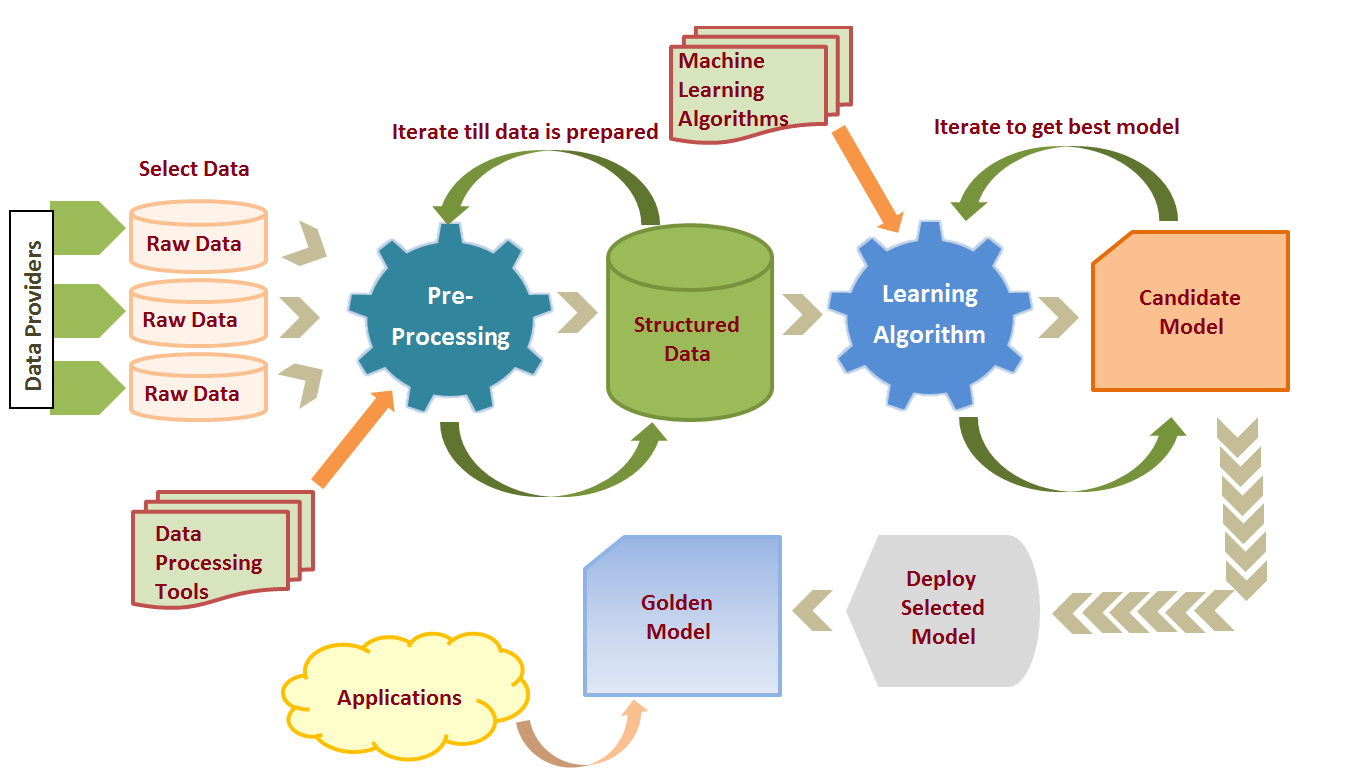
\includegraphics[width=4in, height=3in]{ML.png}}
\caption{Steps in learning a machine}
\end{figure}


\end{frame}
\begin{frame}
\frametitle{Types of machine learning?}
\begin{figure}
\framebox{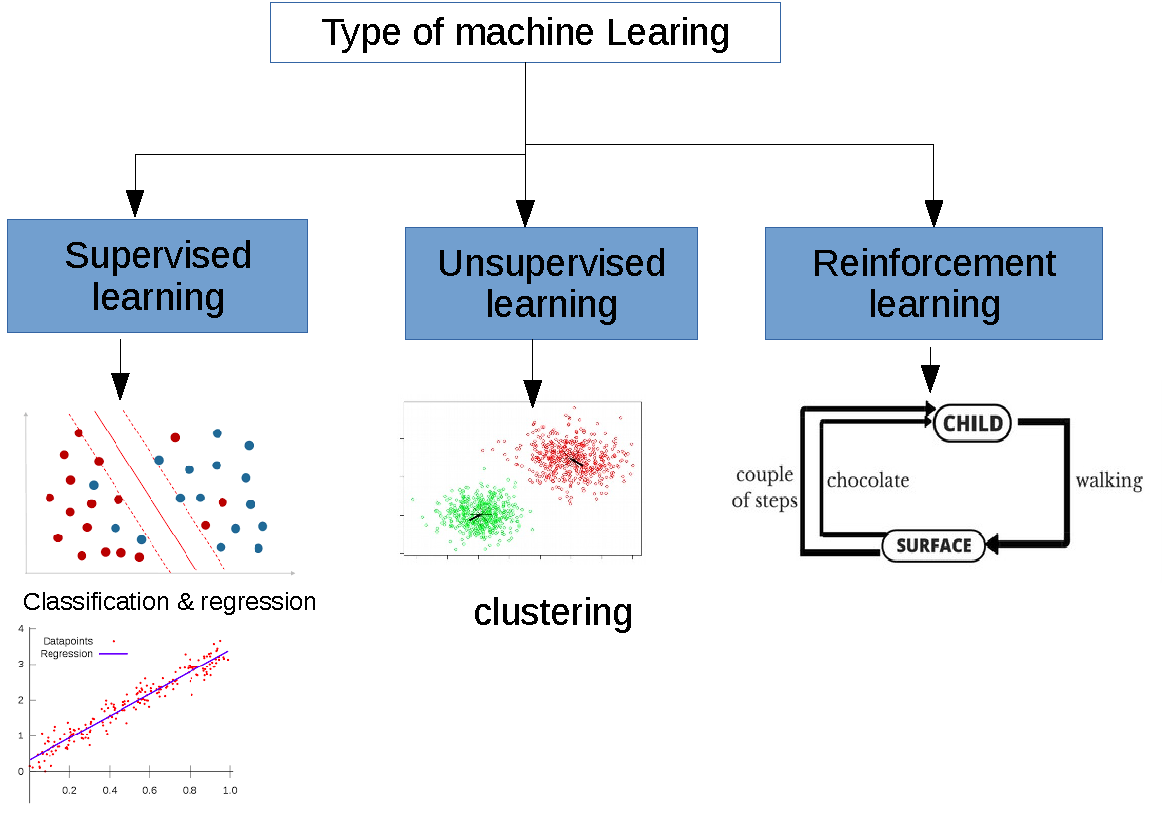
\includegraphics[width=4in, height=3in]{typespdf-crop.pdf}}

\end{figure}


\end{frame}

%\section{Logistic regression}


%\begin{frame}
%\frametitle{Contd...}
%
%\begin{figure}
%\framebox{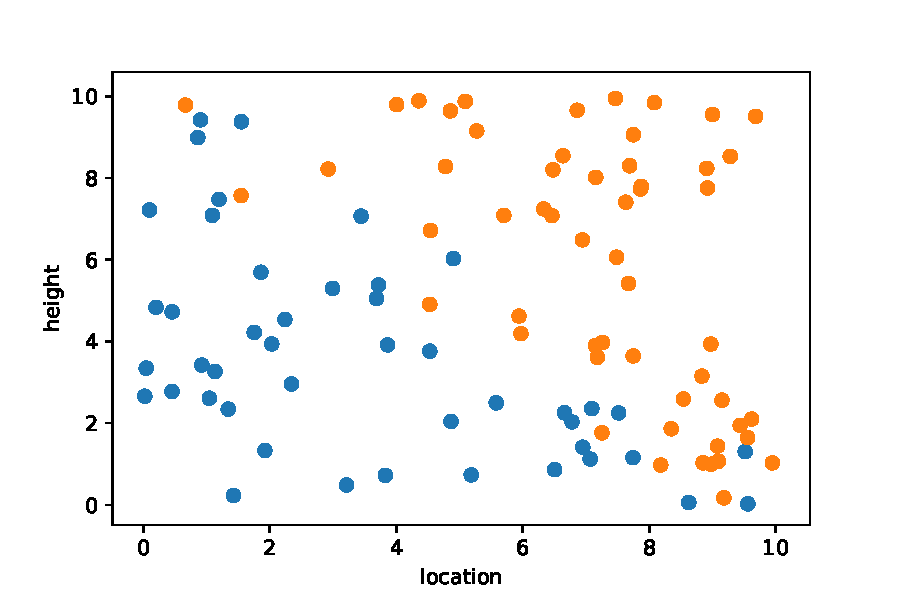
\includegraphics[width=2in, height=2in]{scatter.pdf}}
%\caption{Binary class data}
%\end{figure}
%\end{frame}
%
%\begin{frame}
%\frametitle{Contd...}
%\frametitle{Logistic function aka sigmoid function}
%
%\end{frame}


\end{document}
